Analyses of the dynamics of brain models can provide an understanding of the mechanisms underlying a wide variety of brain behaviors.
Multistability and bifurcations can be interpreted as being at the center of many different states, from seizures to switching from syncopated to anti-syncopated finger tapping \cite{Wang2012,Jirsa2014,Santos2017,Baier2012,Breakspear2005,Jirsa2014,Breakspear2017}.
With that in mind, it is worthwhile to look at some examples of bifurcation analyses of neural models.
\subsection{The Wilson-Cowan Model}
\label{sec:lit_review_bifurcation_wc}
One of the simplest models which lends itself to bifurcation analysis is the Wilson-Cowan model (\cref{eq:wc_x,eq:wc_y,eq:wc_z}).
Traces of $x$ over time look remarkably like the output from an EEG scan.
\Cref{fig:wc_and_swe} shows a simulation of the Wilson-Cowan model with the parameters\footnote{Parameters taken from \cite{Wang2012}, table 1.  Note that the values in rows 3(g),3(i) and 3(j),3(l) should be switched.}:
\begin{equation}
  \label{eq:wc_params}
  C
  =
  \bmqty{23 & -15 & -10 \\ 35 & 0 & 0 \\ 10 & 0 & 0}
  \qc
  \bmqty{P \\ Q \\ R}
  =
  \bmqty{3 \\ -5 \\ -5}
  \qc
  \tau
  =
  \bmqty{0.015 \\ 0.013 \\ 0.267}
\end{equation}
These results show a stereotypical spike-wave event, represented to a high degree of accuracy relative to the simplicity of the model.
\begin{figure}[ht]
  \centering
  \begin{subfigure}{0.5\textwidth}
    \centering
    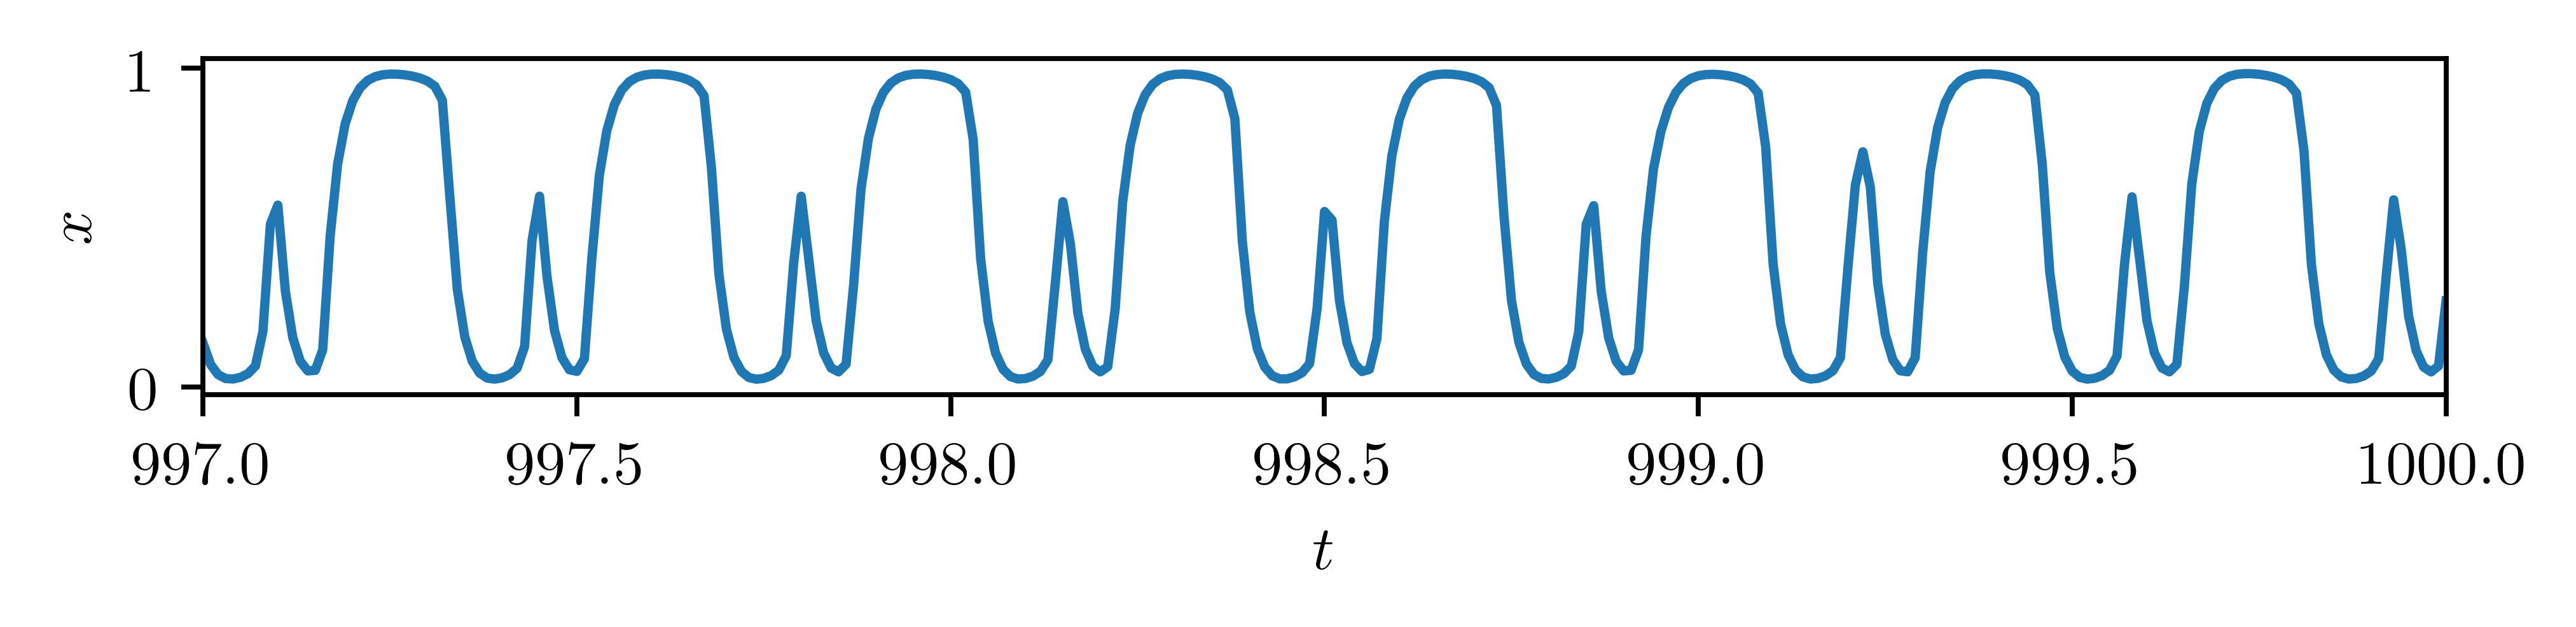
\includegraphics[width=\textwidth]{figure/wc}
    \caption[Wilson-Cowan simulation]{}
    \label{fig:wc}
  \end{subfigure}%
  \begin{subfigure}{0.5\textwidth}
    \centering
    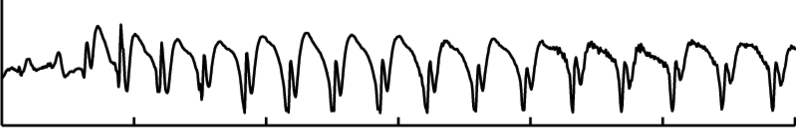
\includegraphics[width=\textwidth]{figure/swe}
    \caption[Spike-wave event]{}
    \label{fig:swe}
  \end{subfigure}
  \caption[Wilson-Cowan simulation and spike-wave event]{A comparison of a simulation of the Wilson-Cowan system and an actual EEG trace of spike-wave event.
    (a) The output of a simulation of the Wilson-Cowan model (\cref{eq:wc_x,eq:wc_y,eq:wc_z}) using parameters from \cite{Wang2012}.
    A 4th-order Runge-Kutta solver ($\dd{t} = 0.01$, $t_{\text{max}} = 1000$) was run on the Wilson-Cowan model with parameters shown in \cref{eq:wc_params}.
    (b) An EEG trace of a spike-wave event, often characteristic of absence seizures.
    Taken and modified from \cite{Marten2009}.
  }
  \label{fig:wc_and_swe}
\end{figure}

The main challenge to performing bifurcation analysis on this type of system is two-fold.
The first aspect is that there are 15 parameters to vary.
This makes bifurcation analysis exceedingly difficult, as all 15 dimensions and their relationships to each other must be analyzed.
This is closely related to the second aspect of the challenge this model provides: the variables in this model are abstracted from their physical/physiological meanings.
For example, because the coupling strengths do not correspond directly to any measurable values, it is hard to gain actionable semantic knowledge from analysis of their effects on the system \cite{Jirsa2014}.

However, it is possible to observe a bifurcation if the external input $P$ varies (\cref{eq:wc_x}).
\Cref{fig:wc_bifurcation} shows the change from spike-wave behavior to simple wave behavior as $P$ increases past 3.92, at time 47.3.
While it would be impossible to do an exhaustive sweep of parameter space, one can observe all of the dynamics of brain behavior in this model.
\begin{figure}[ht]
  \centering
  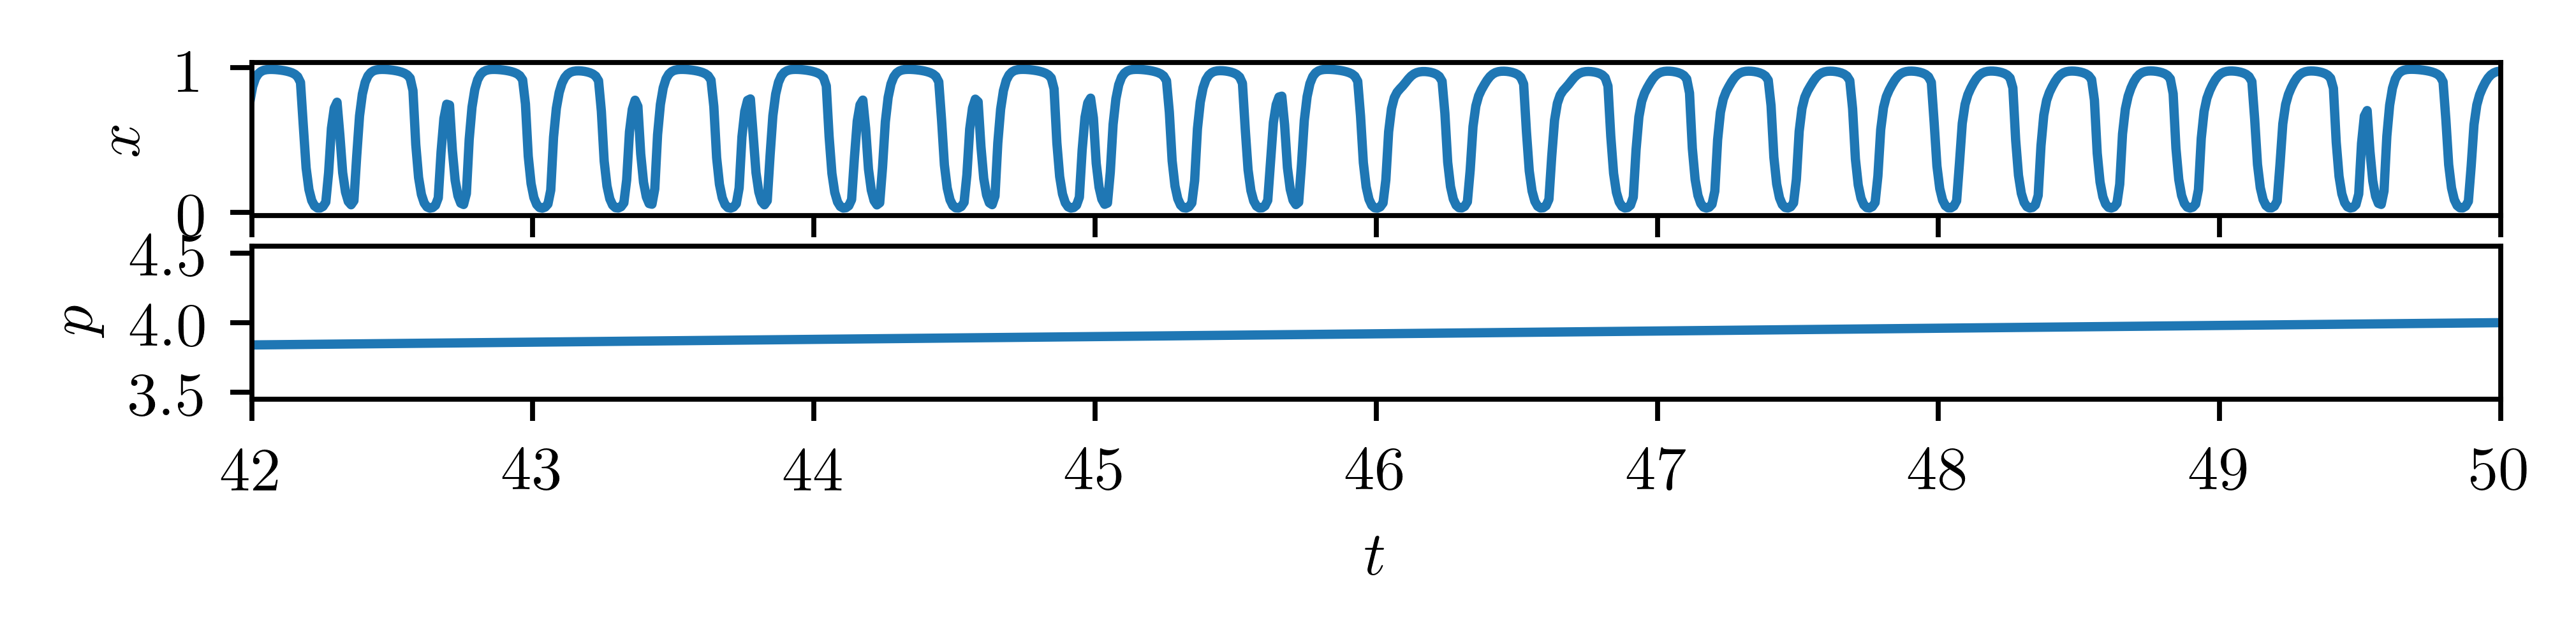
\includegraphics{figure/wc_bifurcation}
  \caption[Wilson-Cowan bifurcation]{A bifurcation from spike-wave behavior to simple wave behavior in the Wilson-Cowan model as a function of continuously varying external input parameter $P$.
    Simulation used a 4th-order Runge-Kutta solver ($\dd{t} = 0.01$, $t_{max} = 100$) as $P$ linearly increased from 3 to 5.
  }
  \label{fig:wc_bifurcation}
\end{figure}

\subsection{The Epileptor Model}
\label{sec:lit_review_bifurcation_epileptor}
In the Epileptor model (\cref{eq:epileptor_x1,eq:epileptor_y1,eq:epileptor_z,eq:epileptor_x2,eq:epileptor_y2,eq:epileptor_f1,eq:epileptor_f2,eq:epileptor_g}), bifurcations depending on the slow permittivity variable $z$ determine whether the brain is behaving normally, or having a seizure \cite{Jirsa2014}.
Given the time scale on which $z$ varies ($\frac{1}{2857}$ times as fast as $x_{1}$) and the bifurcations' dependence on it, it acts like an external parameter to the system, causing the model to go into and out of seizure.
In \cref{fig:epileptor}, the transitions into and out of seizure are clear as critical points in $z$.
Particularly, as is the case with many similar models, normal steady-state brain function corresponds to a stable fixed point, while seizure-like events are on stable limit cycles.
This raises the question: what kinds of bifurcations occur during the transition from healthy brain activity to seizures and back?
\begin{figure}[ht]
  \centering
  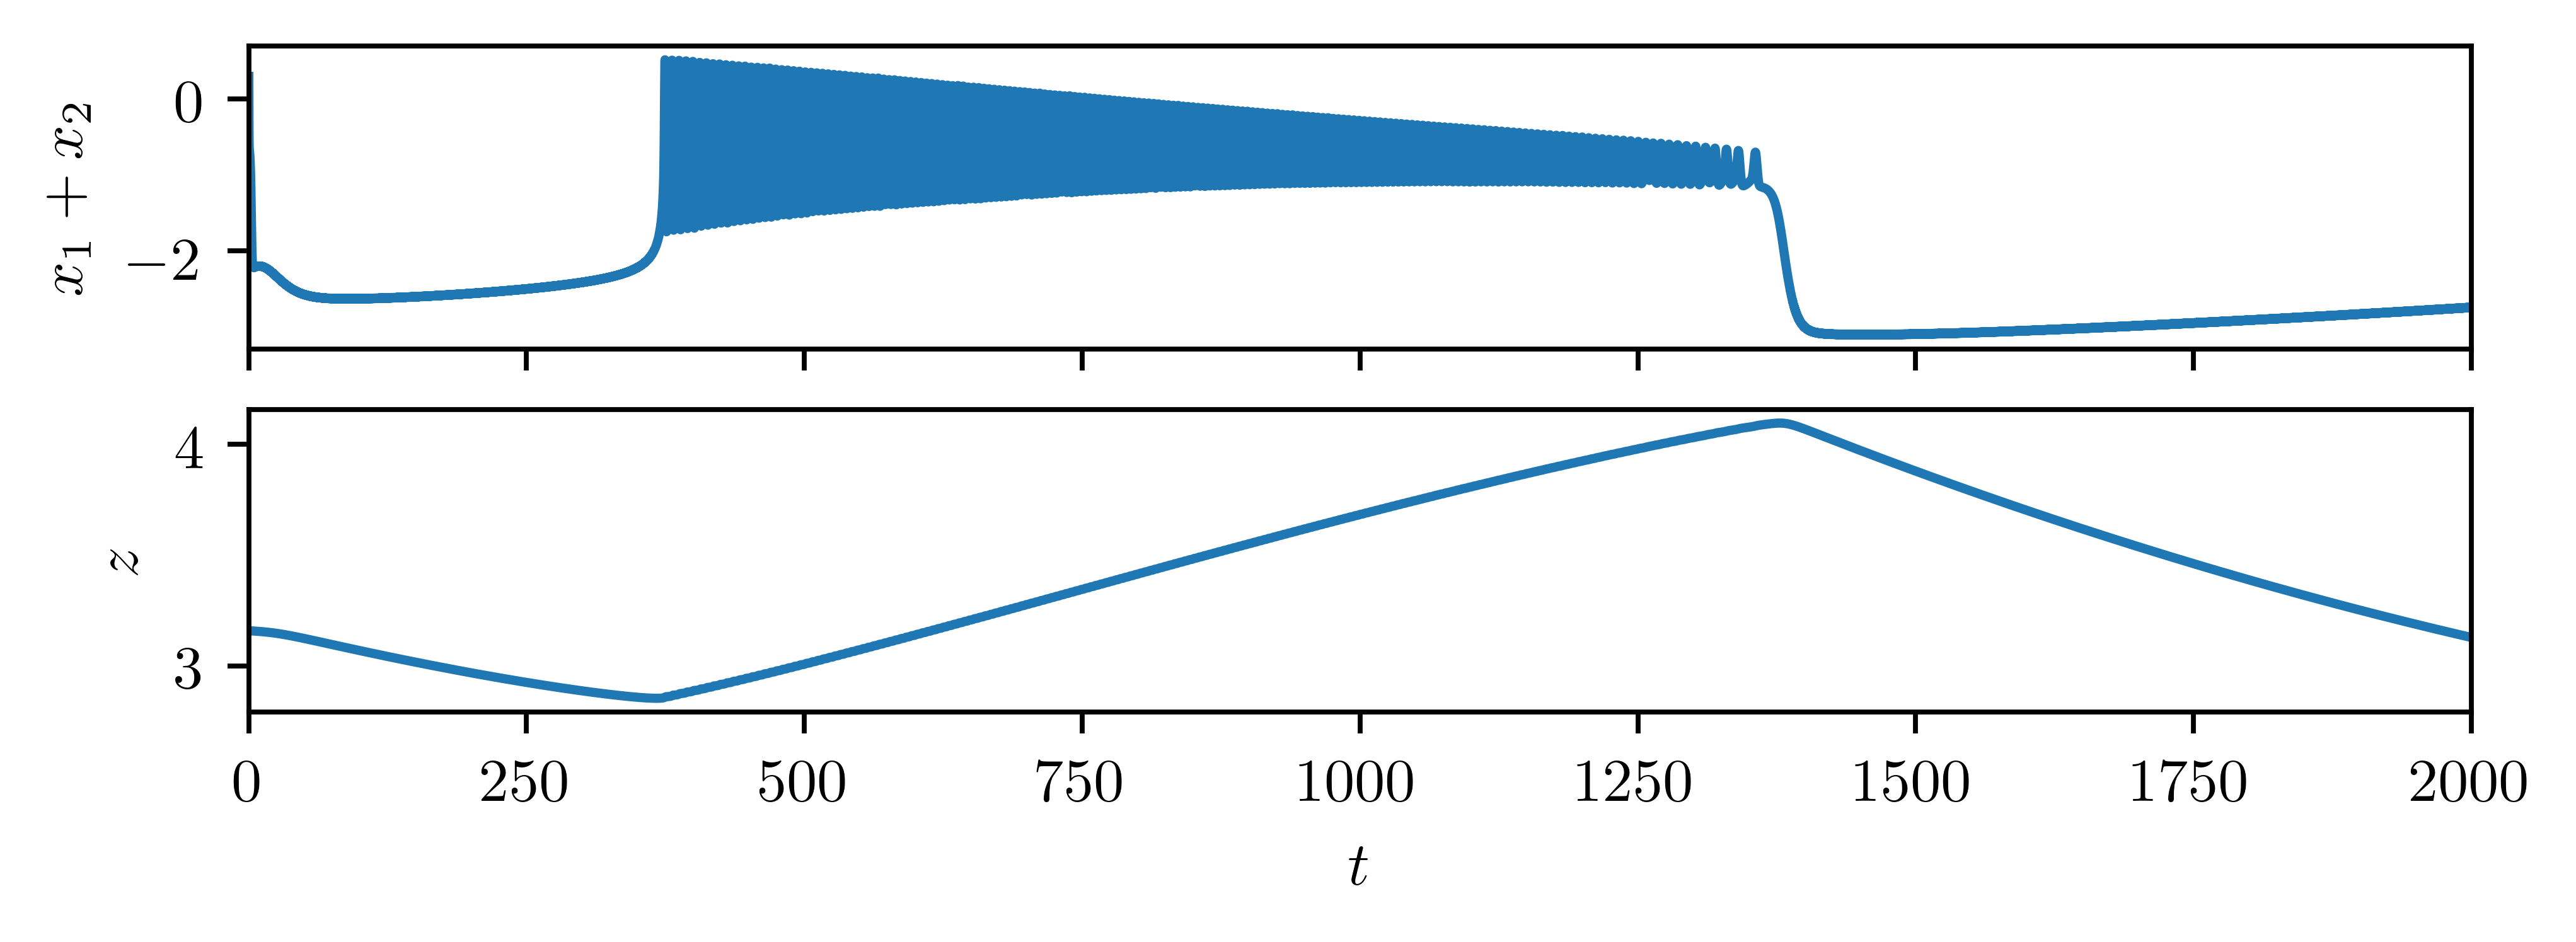
\includegraphics{figure/epileptor}
  \caption[Epileptor simulation]{A simulation of the Epileptor model showing the observable $x_{1}$ and the slow-changing permittivity variable $z$, using a 4th-order Runge-Kutta solver ($\dd{t} = 0.01$, $t_{\text{max}} = 2000$) and the parameters listed in \cref{sec:intro_seizures_aetiology_epileptor}.
    The brain is exhibiting healthy behavior for $t \in \pqty{0, 360} = h_{1}$, then rapidly jumps into a seizure-like behavior.
    It stays in this state for $t \in \pqty{360, 1360} = s$, until it returns to a healthy fixed point for $t \in \pqty{1360, 2000} = h_{2}$.
    Note the DC shift, wherein $x_{1}(s) > x_{1}(h_{1}) \approx x_{1}(h_{2})$.
  }
  \label{fig:epileptor}
\end{figure}

To discuss the dynamics of Epileptor in general, we will use the stereotypical behavior displayed in \cref{fig:epileptor}.
An important aspect of epileptor to note is that $x_{1} + x_{2}$ is the closest variable to an observable quantity, but it still does not resemble an EEG trace without some post-processing.
Particularly, $x_{1}$ would look a lot more like the output from an EEG if put through a high-pass filter.
However, there is an invertible map directly between $x_{1} + x_{2}$ and the readings from an EEG, so the results can be treated as the same \cite{Jirsa2014}.

During seizure onset at $t = 360$, the stable fixed point of healthy activity disappears, replaced by a stable limit cycle.
This indicates that the system undergoes either a Hopf or a saddle-node bifurcation.
A hint towards the type of bifurcation involved is that seizures occur suddenly \cite{Kandel2013}.
This means that the amplitude of oscillation does not steadily increase from 0, meaning that a supercritical Hopf bifurcation can be ruled out \cite{Strogatz2015}.
At $t = 360$, the mean values of $x_{1} + x_{2}$ jump from $\expval{x_{1}(t) + x_{2}(t)}_{t \in h_{1}} = -2.5$ to $\expval{x_{1}(t) + x_{2}(t)}_{t \in s} = -0.8$.
This DC shift does appear in experiment, and indicates that the bifurcation can not be a subcritical Hopf.
This leaves only a saddle-node bifurcation for the transition into a seizure \cite{Jirsa2014}.

As the seizure ends at $t = 1360$, the model returns from a limit cycle to a fixed point with another DC shift.
This indicates that the bifurcation is either a fold bifurcation or a homoclinic bifurcation.
One important point of note is that the frequency of oscillation decreases as the seizure approaches offset, which matches with experiment.
This indicates that the transition must be a homoclinic bifurcation, because systems maintain constant frequency as they approach fold bifurcations \cite{Jirsa2014}.

%%% Local Variables:
%%% mode: latex
%%% TeX-master: "../../main"
%%% End:
